%**************************************************************************************
% License:
% CC BY-NC-SA 4.0 (http://creativecommons.org/licenses/by-nc-sa/4.0/)
%**************************************************************************************

\documentclass[notes]{beamer}

\mode<presentation> {

\usetheme{Madrid}

% Burnt orange
\definecolor{burntorange}{rgb}{0.8, 0.33, 0.0}
\colorlet{beamer@blendedblue}{burntorange}
% Pale yellow
\definecolor{paleyellow}{rgb}{1.0, 1.0, 0.953}
\setbeamercolor{background canvas}{bg=paleyellow}
% Secondary and tertiary palett
\setbeamercolor*{palette secondary}{use=structure,fg=white,bg=burntorange!80!black}
\setbeamercolor*{palette tertiary}{use=structure,fg=white,bg=burntorange!60!black}

% To remove the footer line in all slides uncomment this line
%\setbeamertemplate{footline}
% To replace the footer line in all slides with a simple slide count uncomment this line
%\setbeamertemplate{footline}[page number]

% To remove the navigation symbols from the bottom of all slides uncomment this line
%\setbeamertemplate{navigation symbols}{}
}

\usepackage{amsmath}
\usepackage{bm}
\usepackage{breqn}
\usepackage{cancel}
\usepackage{graphicx} % for figures
\usepackage{subcaption} % for subplots 
\usepackage[labelsep=space,tableposition=top]{caption}
\renewcommand{\figurename}{Fig.} 
\usepackage{cleveref}
\usepackage{caption,subcaption}% http://ctan.org/pkg/{caption,subcaption}
\usepackage{booktabs} % Allows the use of \toprule, \midrule and \bottomrule in tables
\usepackage{multirow}
\usepackage{tabularx}
\usepackage{siunitx}
\usepackage{cleveref}
\usepackage{xcolor}
\usepackage{empheq}
\usepackage[most]{tcolorbox}

\newtcbox{\mymath}[1][]{%
	nobeforeafter, math upper, tcbox raise base,
	enhanced, colframe=blue!30!black,
	colback=blue!30, boxrule=1pt,
	#1}

% To print 2 slides on a page
%\usepackage{handoutWithNotes}
%\pgfpagesuselayout{2 on 1}[border shrink=2mm]
%----------------------------------------------------------------------------------------
%	TITLE PAGE
%----------------------------------------------------------------------------------------
% The short title appears at the bottom of every slide, the full title is only on the title page
\title[CE394M: Cam-Clay]{CE394M: Critical State and Cam-Clay} 
\author{Krishna Kumar} % name
\institute[UT Austin] % institution 
{
University of Texas at Austin \\
\medskip
\textit{
  \url{krishnak@utexas.edu}} % Your email address
}
\date{\today} % Date, can be changed to a custom date

\begin{document}

\begin{frame}
\titlepage % title page as the first slide
\end{frame}

\begin{frame}
 % Table of contents slide, comment this block out to remove it
 \frametitle{Overview}
  %Throughout your presentation, if you choose to use \section{} and \subsection{} 
  %commands, these %will automatically be printed on this slide as an overview 
 \tableofcontents
\end{frame}

%----------------------------------------------------------------------------------------
% slides
%----------------------------------------------------------------------------------------
\section{Critical State Soil Mechanics}
%----------------------------------------------------------------------------------------
\begin{frame}
\frametitle{Critical State Soil Mechanics}
Roscoe et al., (1958), Schofield \& Worth (1968), Wood (1990):
\mode<beamer>{
	\begin{itemize}
		\item Provides a conceptual framework in which to interpret stress-strain-strength-volumetric strain response of soil.
		\item Started as a qualitative, rather than a mathematical model
		\item A unified framework of known or observed soil responses: drained / undrained / etc
	\end{itemize}
}
\mode<handout>{
	\vspace{6cm}
}
\end{frame}

%----------------------------------------------------------------------------------------
\begin{frame}
\frametitle{Critical state variables}
\noindent
\fboxsep=0pt
\noindent
\begin{minipage}[t]{0.65\linewidth}
	\begin{itemize}
		\item Mean stress: $p^\prime = \frac{\sigma_a^\prime  + 2 \sigma_r^\prime}{3} = p - u$.
		\item Deviatoric stress: $q = \sigma_a^\prime - \sigma_r^\prime = \sigma_a - \sigma_r$
		\mode<beamer>{
			\item Specific volume: $v = \frac{V_T}{V_s} = \frac{V_s + V_v}{V_s} = 1 + e$.
		}
		\mode<handout>{
			\vspace{1cm}
		}	
		
	\end{itemize}
\end{minipage}%
\hfill
\begin{minipage}[t]{0.35\linewidth}
	\begin{figure}
	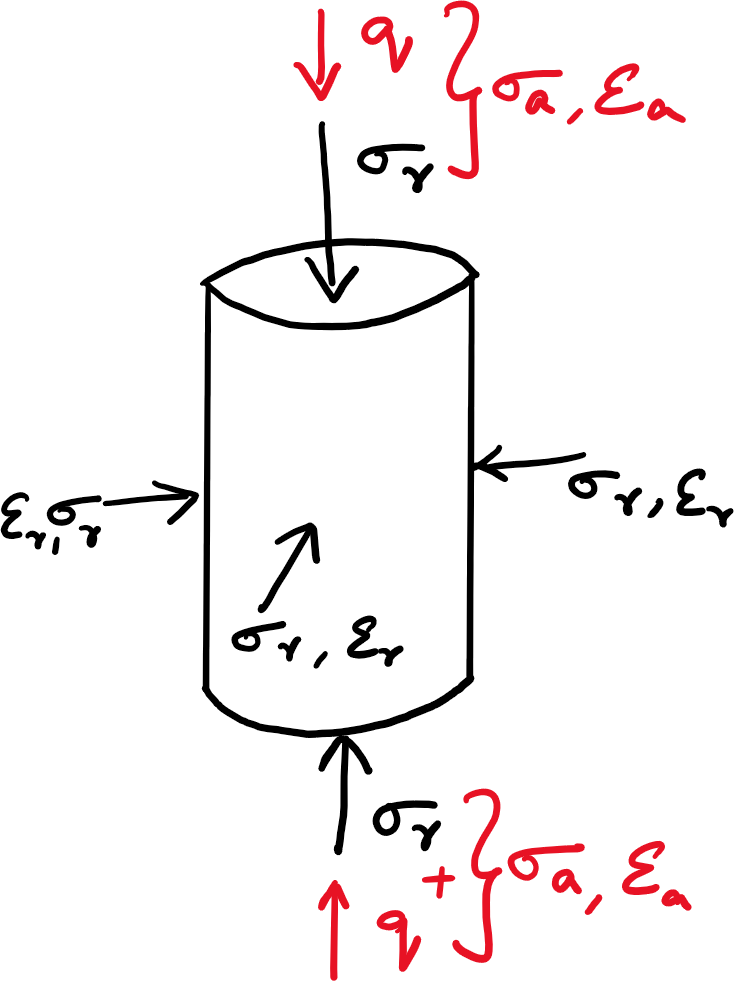
\includegraphics[width=0.9\textwidth]{figs/triaxial.png}
	\end{figure}
\end{minipage}	
\end{frame}

%----------------------------------------------------------------------------------------
\begin{frame}
\frametitle{Critical State Hypothesis: I}
Roscoe, Schofield \& Worth (1958): \textbf{At shear-failure, soil exists at a unique state}
\mode<beamer>{
	\begin{itemize}
		\item $d\varepsilon_q >> 0$ unlimited shear strain potential.
		\item $dp^\prime = dq = d\varepsilon_p = 0$ no change in $p^\prime, q, \varepsilon_p$.
		\item Critical state stress ratio: $\eta = q / p^\prime = const = M$ at failure $q = M p^\prime$.
	\end{itemize}
}
\mode<handout>{
	\vspace{3cm}
}
\begin{figure}
	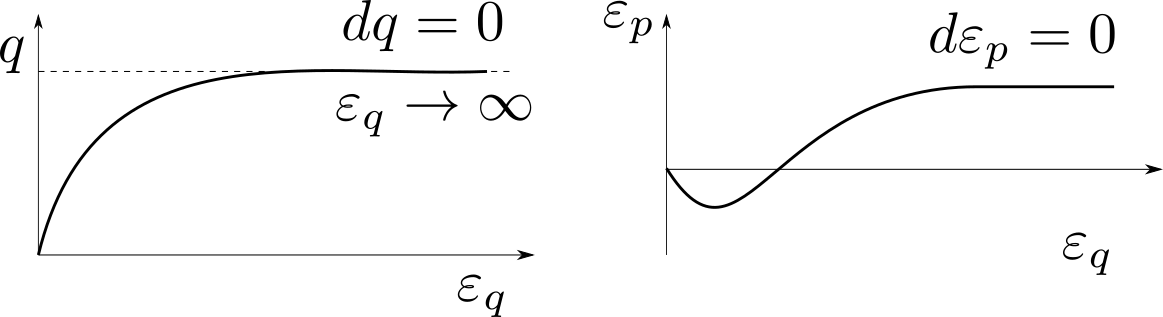
\includegraphics[width=0.9\textwidth]{figs/critical-state.png}
\end{figure}
\end{frame}
\note{Soil is sheared to a point where stresses are stationary $(dq = dp^\prime = 0)$ with no futher change in volume $(d\varepsilon_p = 0)$, unlimited shear strains $(d\varepsilon_q >> 0)$ and $q/p^\prime$ has a fixed value: \textbf{critical state}.

$M$ can be related to $phi^\prime$: $M = \frac{6\sin\phi^\prime}{3 - \sin\phi^\prime}$.
}


%----------------------------------------------------------------------------------------
\begin{frame}
\frametitle{Critical State Hypothesis: II}
\textbf{Critical state is a function of $q, p^\prime, v$. }
\begin{figure}
	\includegraphics[width=0.4\textwidth]{figs/critical-state-3d.png}
	\caption*{The CSL ($p^\prime, v, q$) space is given by the intersection of two planes: $q = Mp^\prime$ and a cruved vertical plane $v = \Gamma - \lambda \ln p^\prime$}
\end{figure}
\end{frame}

\note{Critical state curve connecting critical state points:
\begin{itemize}
	\item Crticial state line
	\item Defined in 3D but we'll look at projections into $q - p^\prime$ and $v - p^\prime$ space
\end{itemize}
}


%----------------------------------------------------------------------------------------
\begin{frame}
\frametitle{Critical State Hypothesis: II}
\textbf{Critical state is a function of $q, p^\prime, v$. }
\begin{figure}
	\includegraphics[width=\textwidth]{figs/critical-state-2d.png}
	\caption*{The CSL in (a) ($p^\prime, q$) plot and (b) ($p^\prime, v$) plot (isotropic normal compression line is shown in dashed)}
\end{figure}
\end{frame}

%----------------------------------------------------------------------------------------
\begin{frame}
\frametitle{Critical State Hypothesis: II}
\textbf{Critical state is a function of $q, p^\prime, v$. }
\begin{figure}
	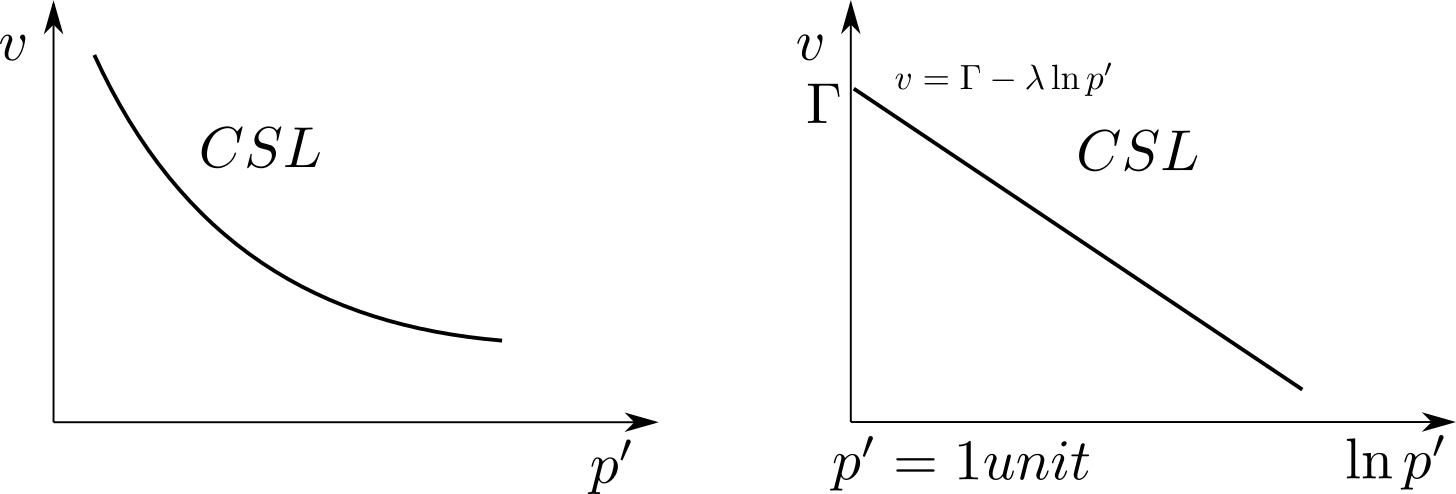
\includegraphics[width=\textwidth]{figs/v-lnp.png}
\end{figure}
\end{frame}

%----------------------------------------------------------------------------------------
\begin{frame}
\frametitle{Critical State Hypothesis: II}
\textbf{Critical state is a function of $q, p^\prime, v$. }
\begin{figure}
	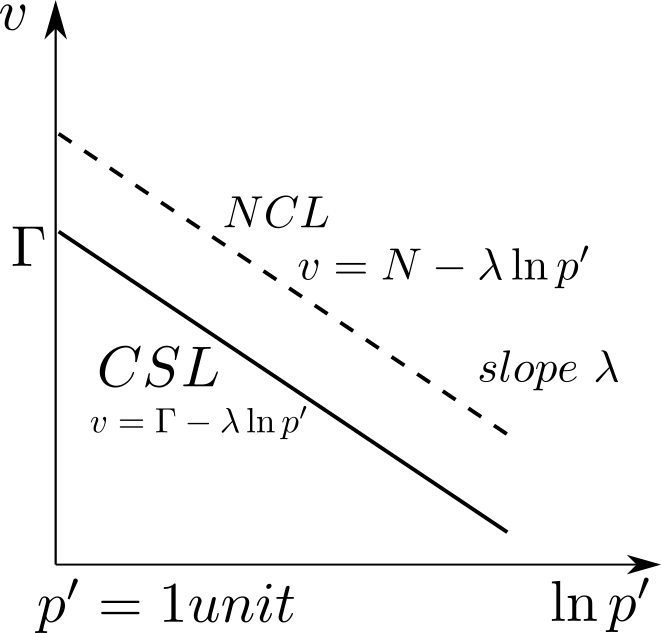
\includegraphics[width=0.6\textwidth]{figs/csl-ncl.png}
\end{figure}
\end{frame}

\note{
	Isotropic virgin compression line (VCL) $\eta = 0$. NCL is parallel to CSL. VCL is $\eta = 0$, while CSL $\eta = M$. Oedometer falls between VCL and CSL at a constant $\eta$: $0 < \eta < M$.
}


%----------------------------------------------------------------------------------------
\begin{frame}
\frametitle{Critical State Hypothesis: II}
\textbf{Critical state is a function of $q, p^\prime, v$. }
\begin{figure}
	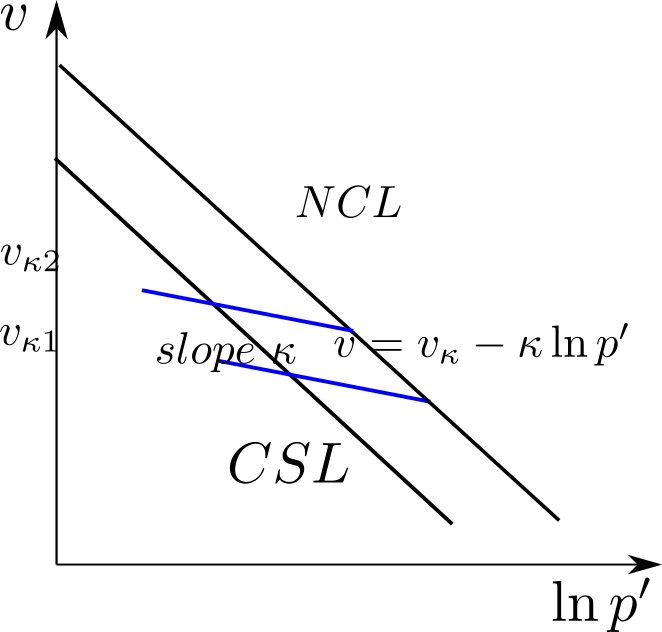
\includegraphics[width=0.65\textwidth]{figs/kappa.png}
\end{figure}
\end{frame}

\note{$v_\kappa$ depends on which $\kappa$ line you are on. $\kappa \ne c_r$ and $\lambda \ne C_c$}


%----------------------------------------------------------------------------------------
\begin{frame}
\frametitle{Stress paths $\sigma_3^\prime / \sigma_1^\prime = K_c = const$}
\begin{figure}
	\includegraphics[width=0.54\textwidth]{figs/stress-paths-kc.png}
\end{figure}
\end{frame}

%----------------------------------------------------------------------------------------
\begin{frame}
\frametitle{Clay behavior}
\begin{figure}
	\includegraphics[width=0.7\textwidth]{figs/clay-behavior.png}
\end{figure}
\end{frame}

%----------------------------------------------------------------------------------------
\begin{frame}
\frametitle{Critical state boundary surface}
\begin{figure}
	\includegraphics[width=0.45\textwidth]{figs/yieldsurface-3d.png}
\end{figure}
\end{frame}

%----------------------------------------------------------------------------------------
\begin{frame}
\frametitle{Summary of critical state behavior}
\mode<beamer>{
	\begin{itemize}
		\item Can only traverse NCL in one direction
		\item Can traverse RCL ($\kappa$-line) in both directions
		\item To move from one $\kappa$-line to another must move along NCL. Hence, plastic volumetric strains must occur.
		\item Critical state line is \textbf{NOT} a yield surface. It's where it's going but a lot of plastic straining is needed to get there. (if $CSL = F = 0$) then with associative flow rule $d\varepsilon_p^p \ne0$ at critical state. Real $F$ is horizontal at critical state.
	\end{itemize}
}
\mode<handout>{
	\vspace{6cm}
}
\end{frame}


%----------------------------------------------------------------------------------------
\section{Cam-Clay}

%----------------------------------------------------------------------------------------

%----------------------------------------------------------------------------------------
\begin{frame}
\frametitle{Stress - dilatancy theory (Taylor, 1948)}
\begin{figure}
	\includegraphics[width=0.45\textwidth]{figs/direct-shear.png}
\end{figure}
\mode<beamer>{
	Work in friction and dilation:
	\begin{equation*}
		\tau dx - \sigma_n^\prime dy = \mu \sigma_n^\prime dx
	\end{equation*}
}
\mode<handout>{
	\vspace{3cm}
}
\end{frame}

\note{Taylor (1948) proposed
	a stress-dilatancy theory based on the work balance equation: The external work
	corresponds to the product of the measured displacements and forces (assuming that the elastic
	deformation is negligible). The internal work corresponds to the frictional force.}


%----------------------------------------------------------------------------------------
\begin{frame}
\frametitle{Formulation of elasto-plastic Cam-Clay (OCC): Yield function}
Derived from work consideration:
\begin{figure}
	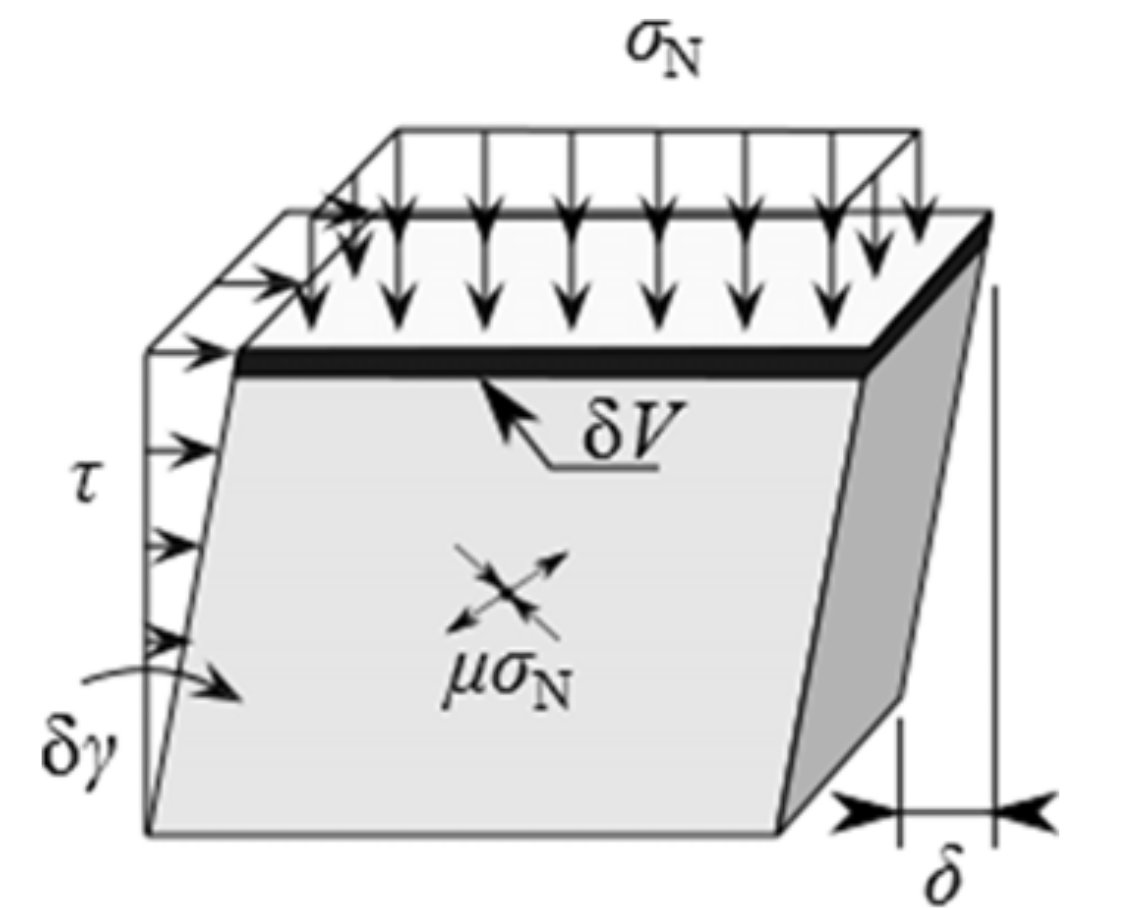
\includegraphics[width=0.4\textwidth]{figs/simple-shear.png}
\end{figure}

\mode<beamer>{
	External work: $\delta w_{ext}^p = p^\prime d\varepsilon_p^p + q d \varepsilon_q^p$
	Assume that the internal work is dissipated by internal friction only: $\delta w_{int}^p = M p^\prime d \varepsilon_q^p$

	\begin{equation*}
		\delta w_{ext}^p = p^\prime d\varepsilon_p^p + q d \varepsilon_q^p = M p^\prime d \varepsilon_q^p = \delta w_{int}^p
	\end{equation*}
}
\mode<handout>{
	\vspace{3cm}
}
\end{frame}
\note{This dissipation function can be regarded simply as generalisation of Taylor's equation. It should be  noted that both Taylor's equation and Cam-Clay dissipation function equation assume that when   there is some combination of volumechange ($dy$ or $\partial \varepsilon_v$) and of shear distortion ($dx$ or $\partial \varepsilon_s$) it is the shear strain that determines the dissipation rate. The dilation or volume change is a geometrical consequence of interlocking, and does not appear explicitly in the dissipation function. }


%----------------------------------------------------------------------------------------
\begin{frame}
\frametitle{Cam-Clay (OCC): Stress dilatancy relation}
\begin{equation*}
p^\prime d\varepsilon_p^p + q d \varepsilon_q^p = M p^\prime d \varepsilon_q^p
\end{equation*}
Rearranging the terms (divide by $p^\prime d\varepsilon_q^p$):
\mode<beamer>{
	\begin{equation*}
	\frac{d\varepsilon_p^p }{d\varepsilon_q^p } = M - \frac{q}{p^\prime} = M - \eta
	\end{equation*}
	Where $\eta = q/p^\prime$ is defined as the stress-ratio. This equation is known as the dilatancy expression and expresses the ratio in plastic volumetric and deviatoric components. 
	
	
	\begin{align*}
	q/p<M: \quad & \frac{d\varepsilon^p_p}{d\varepsilon^p_q} > 0 \rightarrow \quad d\varepsilon^p_p > 0 \quad \text{Contractive response}\\
	q/p > M: \quad &	\frac{d\varepsilon^p_p}{d\varepsilon^p_q} > 0 \rightarrow \quad d\varepsilon^p_p < 0 \quad\text{Dilative response} \\
	q/p = M: \quad & d\varepsilon^p_p  = 0 \quad \text{No volume change}
	\end{align*}
}
\mode<handout>{
	\vspace{6cm}
}
\end{frame}

\note{The critical state is defined by an absence of volume change or, in other words, a nil dilatancy
conditions. Therefore, at critical state, the stress-dilatancy rule yields to the critical state condition $\eta = M$.}


%----------------------------------------------------------------------------------------
\begin{frame}
\frametitle{Cam-Clay (OCC): flow-rule}
The original idea was very simple. The yield locus must be such that each associated flow rule $(\delta \varepsilon_p, \delta \varepsilon_q)$ would be orthogonal to the tangent to the yield locus.

\noindent
\fboxsep=0pt
\noindent
\begin{minipage}[t]{0.65\linewidth}
	\mode<beamer>{
	\begin{equation*}
		\frac{\delta \varepsilon_p}{\delta \varepsilon_q} = - \frac{\delta \varepsilon_q}{\delta \varepsilon_p^\prime}
	\end{equation*}
	From stress dilation condition:
	\begin{equation*}
		\frac{dq}{dp^\prime} = - (M - \eta) = -M + \eta
	\end{equation*}
	Integrating we obtain:
	\begin{equation*}
		q = M p^\prime \ln\left(\frac{p_c^\prime}{p^\prime}\right)
	\end{equation*}
	Where $p^\prime_c$ is the value of $p^\prime$ at $q = 0$.
	}
	\mode<handout>{
		\vspace{4cm}
	}
	
\end{minipage}%
\hfill
\begin{minipage}[t]{0.35\linewidth}
	\begin{figure}
		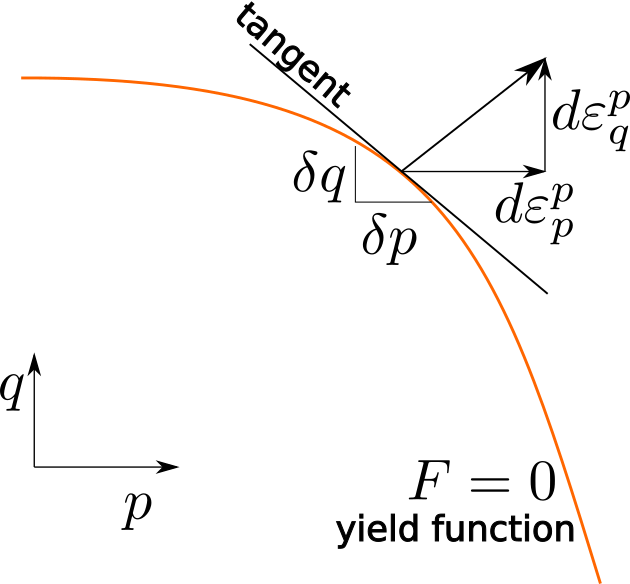
\includegraphics[width=\textwidth]{figs/flow-rule.png}
	\end{figure}
\end{minipage}
\end{frame}

\note{\textbf{Original Cam-Clay integration}
	\begin{equation*}
	\eta = q/p \quad \rightarrow d\eta = \frac{\partial \eta}{\partial q} dq + \frac{\partial \eta}{\partial p^\prime} dp^\prime
	\end{equation*}

Which gives:
	\begin{equation*}
		d\eta = \frac{dq}{p} - \frac{q}{p^2} dp \rightarrow \quad dq = p d\eta + \eta dp
	\end{equation*}

We know from flow rule and orthogonality: $dq = dp (-M + \eta)$

Equating the above 2 equations:
	\begin{align*}
		dp = & p d\eta + \eta dp =  dp (-M + \eta) \\
		& p d \eta = -M dp \rightarrow \quad deta = -M \frac{dp}{p}
	\end{align*}
Integrating this expression we obtain:
	\begin{equation}
		\eta = -M \ln p + C
	\end{equation}
}


\note{\textbf{Original Cam-Clay integration}
	\begin{equation}
	\eta = -M \ln p + C
	\end{equation}
To find the constants, for $\eta = 0$, we get $p = p_c$:
	\begin{equation*}
		0 = -M \ln p_c + C \quad C = M \ln p_c
	\end{equation*}
Which gives:
	\begin{align*}
		\eta &= M \ln p_c - M \ln p \\
		q/p &= M \ln \left(p_c/p\right)
	\end{align*}
Yield function:
	\begin{equation*}
		F = q - M p^\prime \ln(p_c^\prime / p^\prime) = 0
	\end{equation*}
}

%----------------------------------------------------------------------------------------
\begin{frame}
\frametitle{Cam-Clay (OCC): Elastic properties}
\noindent
\fboxsep=0pt
\noindent
\begin{minipage}[t]{0.65\linewidth}
	\mode<beamer>{
		Swelling: $\delta v_\kappa = \kappa \ln (p^\prime_1 /p^\prime_2)$
		
		Elastic bulk modulus: $K = \frac{dp^\prime}{d\varepsilon_p}$.
		
		We know the volumetric compression on elastic reloading line:
		
		$dv = -\kappa \frac{dp^\prime }{p^\prime}$
		
		\begin{equation*}
		d \varepsilon_p = \frac{-de}{1 + e_0} = \frac{-dv}{v_0} = \frac{\kappa}{v_0}\frac{dp^\prime}{p^\prime}
		\end{equation*}
		
		$K^\prime$ is not constant: $K^\prime = K^\prime (p^\prime)$. Assuming a constant poisson ratio: $\nu$, so $G, K$ vary.
		
		\begin{equation*}
			K = \frac{dp}{d\varepsilon_p} = \frac{v_o p^\prime}{\kappa} = \frac{(1+e_0)p^\prime}{\kappa}
		\end{equation*}	
	}
	\mode<handout>{
		\vspace{6cm}
	}
	
\end{minipage}%
\hfill
\begin{minipage}[t]{0.35\linewidth}
	\begin{figure}
		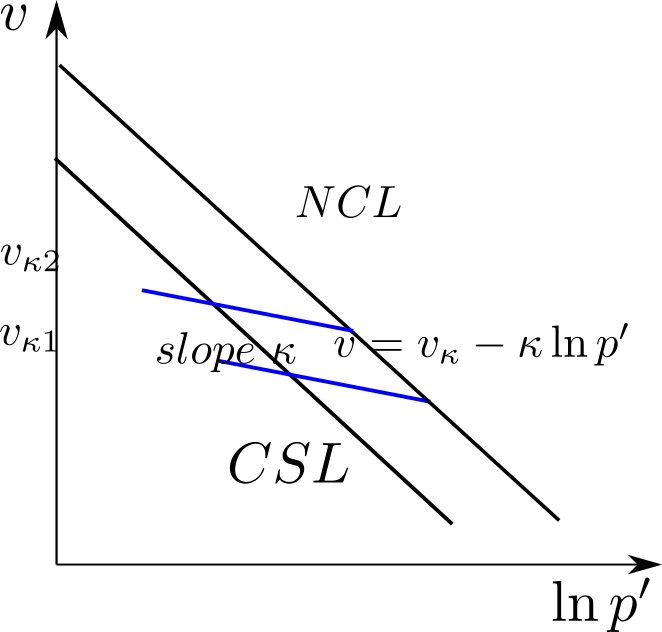
\includegraphics[width=\textwidth]{figs/kappa.png}
	\end{figure}
\end{minipage}
\end{frame}

\note{
	\textit{Observation}: 
	\begin{itemize}
		\item Stiffness $K$ increases with $p^\prime$: correct.
		\item Stiffness increases with void ratio (not right)!
	\end{itemize}
	
	\textit{Note: }The original derivation assumed that there were no recoverable (elastic) shear strains so $G = \infty$. We can find the stress-strain relationships for a single element in this case, but for a finite element forumulation we need to have a finite $G^e$. So there are two options:
	\begin{itemize}
		\item Define $G = f(e, p^\prime)$.
		\item Use a constant ``elastic'' Poisson ratio. Ratio between the shear and bulk modulus is constant. $2G/K = const$.
	\end{itemize}
	The first alternative has the shortcoming that depending on the choice of $G$ we may have unreasonable values of the ``elastic'' Poisson's ratio. I prefer the second choice.
}



%----------------------------------------------------------------------------------------
\begin{frame}
\frametitle{Cam-Clay (OCC): Hardening law}
We need to define how the yield surface hardens as plastic work is being performed. Only ``\textit{memory}'' parameter in our yield surface is the size: $p_c^\prime$.

From the isotropic NCL:
	\begin{equation*}
	d\varepsilon_p = \frac{-dv}{v} = \frac{-de}{1 + e} = \frac{+\lambda}{v} \frac{dp_c^\prime}{p_c^\prime}
	\end{equation*}

But the increment in elastic volumetric strain is:
	\begin{equation*}
	d\varepsilon_p^e = \left(\frac{-dv}{v}\right)^{elastic} = + \frac{\kappa}{v}\left(\frac{dp_c^\prime}{p_c^\prime}\right)
	\end{equation*}
Therefore the increment of $p_c$ can be related to the increment of plastic volumetric strain:
	\begin{equation*}
	d\varepsilon_p^p = 	d\varepsilon_p - 	d\varepsilon_p^e = (\lambda - \kappa)\left(\frac{dp_c^\prime}{p_c^\prime}\right) \rightarrow \quad dp_c^\prime = \left(\frac{v\cdot p_c^\prime}{(\lambda - \kappa)}\right) \cdot d \varepsilon_p^p
	\end{equation*}
\end{frame}



%----------------------------------------------------------------------------------------
\begin{frame}
\frametitle{Cam-Clay (OCC): Hardening law}
We have seen that the hardening law:

\begin{equation*}
H = - \left(\frac{\partial F}{\partial Wp}\right)\left(\frac{\partial Wp}{\partial \varepsilon^p}\right)^T\cdot\frac{\partial G}{\partial \sigma}
\end{equation*}
$W_p$ is the vector of memory parameters. In our case, the CC model has only one parameter:\mode<beamer>{ $p_c^\prime$ and it's variation is only a function of the plastic volumetric strain. So:}
\mode<beamer>{
\begin{equation*}
H = - \left(\frac{\partial F}{\partial p_c^\prime}\right)\left(\frac{\partial p_c^\prime}{\partial \varepsilon^p}\right)^T\cdot\frac{\partial G}{\partial \sigma}
\end{equation*}	
}
\mode<handout>{
\vspace{1cm}
}
\end{frame}



%----------------------------------------------------------------------------------------
\begin{frame}
\frametitle{Cam-Clay (OCC): Hardening law}
We know:
\begin{align*}
\frac{\partial F}{\partial p_c^\prime} & = -M p^\prime / p_c^\prime \\
%
\frac{\partial p_c^\prime}{\partial \varepsilon^p} & = \frac{v}{(\lambda - \kappa)}p^\prime_c \\
%
\frac{\partial G}{\partial \sigma} & = P_p = Q_p = M - \eta
\end{align*}	

\begin{empheq}[box=\tcbhighmath]{equation*}	H = - \left(\frac{\partial F}{\partial p_c^\prime}\right)\left(\frac{\partial p_c^\prime}{\partial \varepsilon^p}\right)^T\cdot\frac{\partial G}{\partial \sigma} = M \frac{(M - \eta)}{(\lambda - \kappa)} \cdot (1 + e) \cdot p^\prime
\end{empheq}	
\end{frame}

\end{document}
